\newpage\pagecolor{black}\color{white}
\section{Andromeda Galaxy}
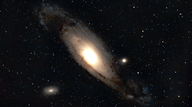
\includegraphics[width=\textwidth]{/home/lcv/Dropbox/AstroPhotography/Imaging/Original/Andromeda_Galaxy.jpg}
{\footnotesize\color{white}
The Andromeda Galaxy is a barred spiral galaxy and is the nearest major galaxy to the Milky Way. It was originally named the Andromeda Nebula and is cataloged as Messier 31, M31, and NGC 224. Andromeda has a D25 isophotal diameter of about 46.56 kiloparsecs (152,000 light-years)[8] and is approximately 765 kpc (2.5 million light-years) from Earth. The galaxy's name stems from the area of Earth's sky in which it appears, the constellation of Andromeda, which itself is named after the princess who was the wife of Perseus in Greek mythology. \myhttp{Wikipedia}{https://en.wikipedia.org/wiki/Andromeda_Galaxy}
}
\section{Bubble Nebula}
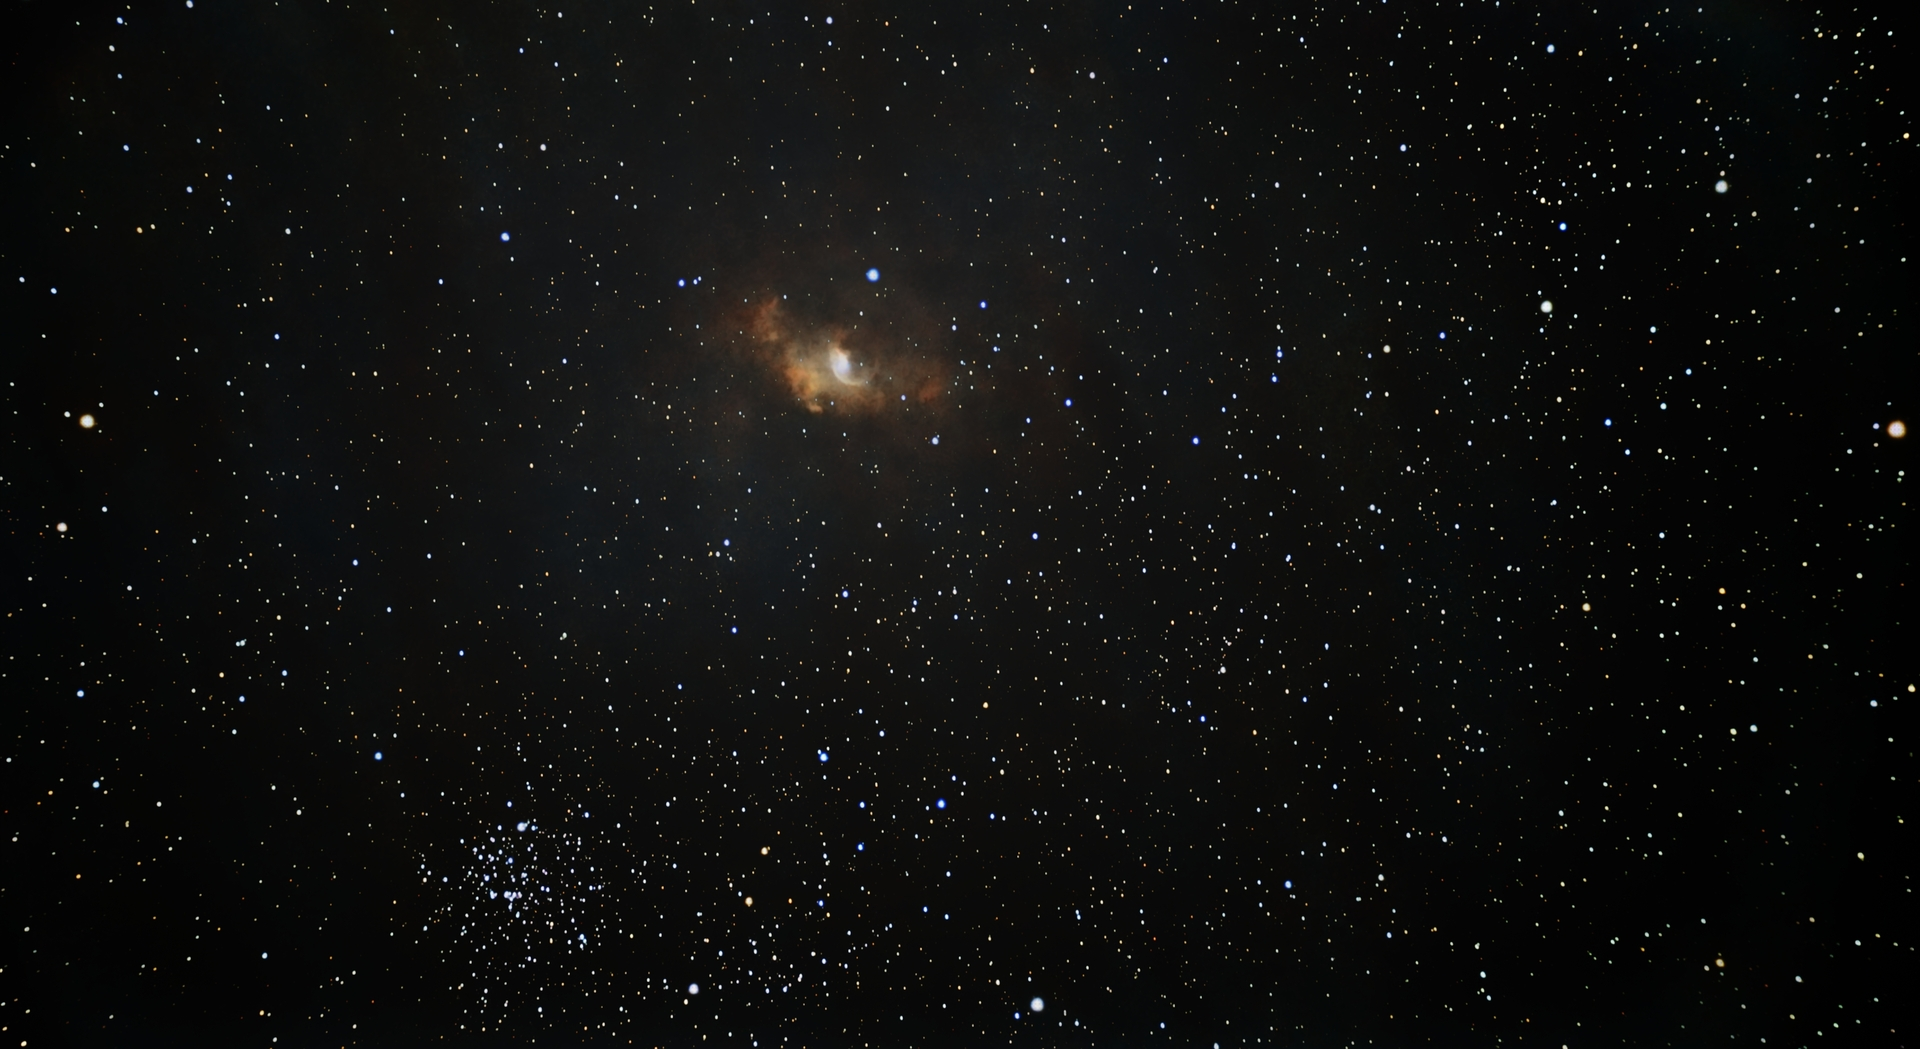
\includegraphics[width=\textwidth]{/home/lcv/Dropbox/AstroPhotography/Imaging/Original/Bubble_Nebula.jpg}
{\footnotesize\color{white}
NGC 7635, also known as the Bubble Nebula, Sharpless 162, or Caldwell 11, is an H II region emission nebula in the constellation Cassiopeia. It lies close to the open cluster Messier 52. The "bubble" is created by the stellar wind from a massive hot, 8.7 magnitude young central star, SAO 20575 (BD+60°2522). The nebula is near a giant molecular cloud which contains the expansion of the bubble nebula while itself being excited by the hot central star, causing it to glow. It was discovered in November 1787 by William Herschel. The star BD+60°2522 is thought to have a mass of about 44 M \myhttp{Wikipedia}{https://en.wikipedia.org/wiki/Andromeda_Galaxy}
}
\section{California Nebula}
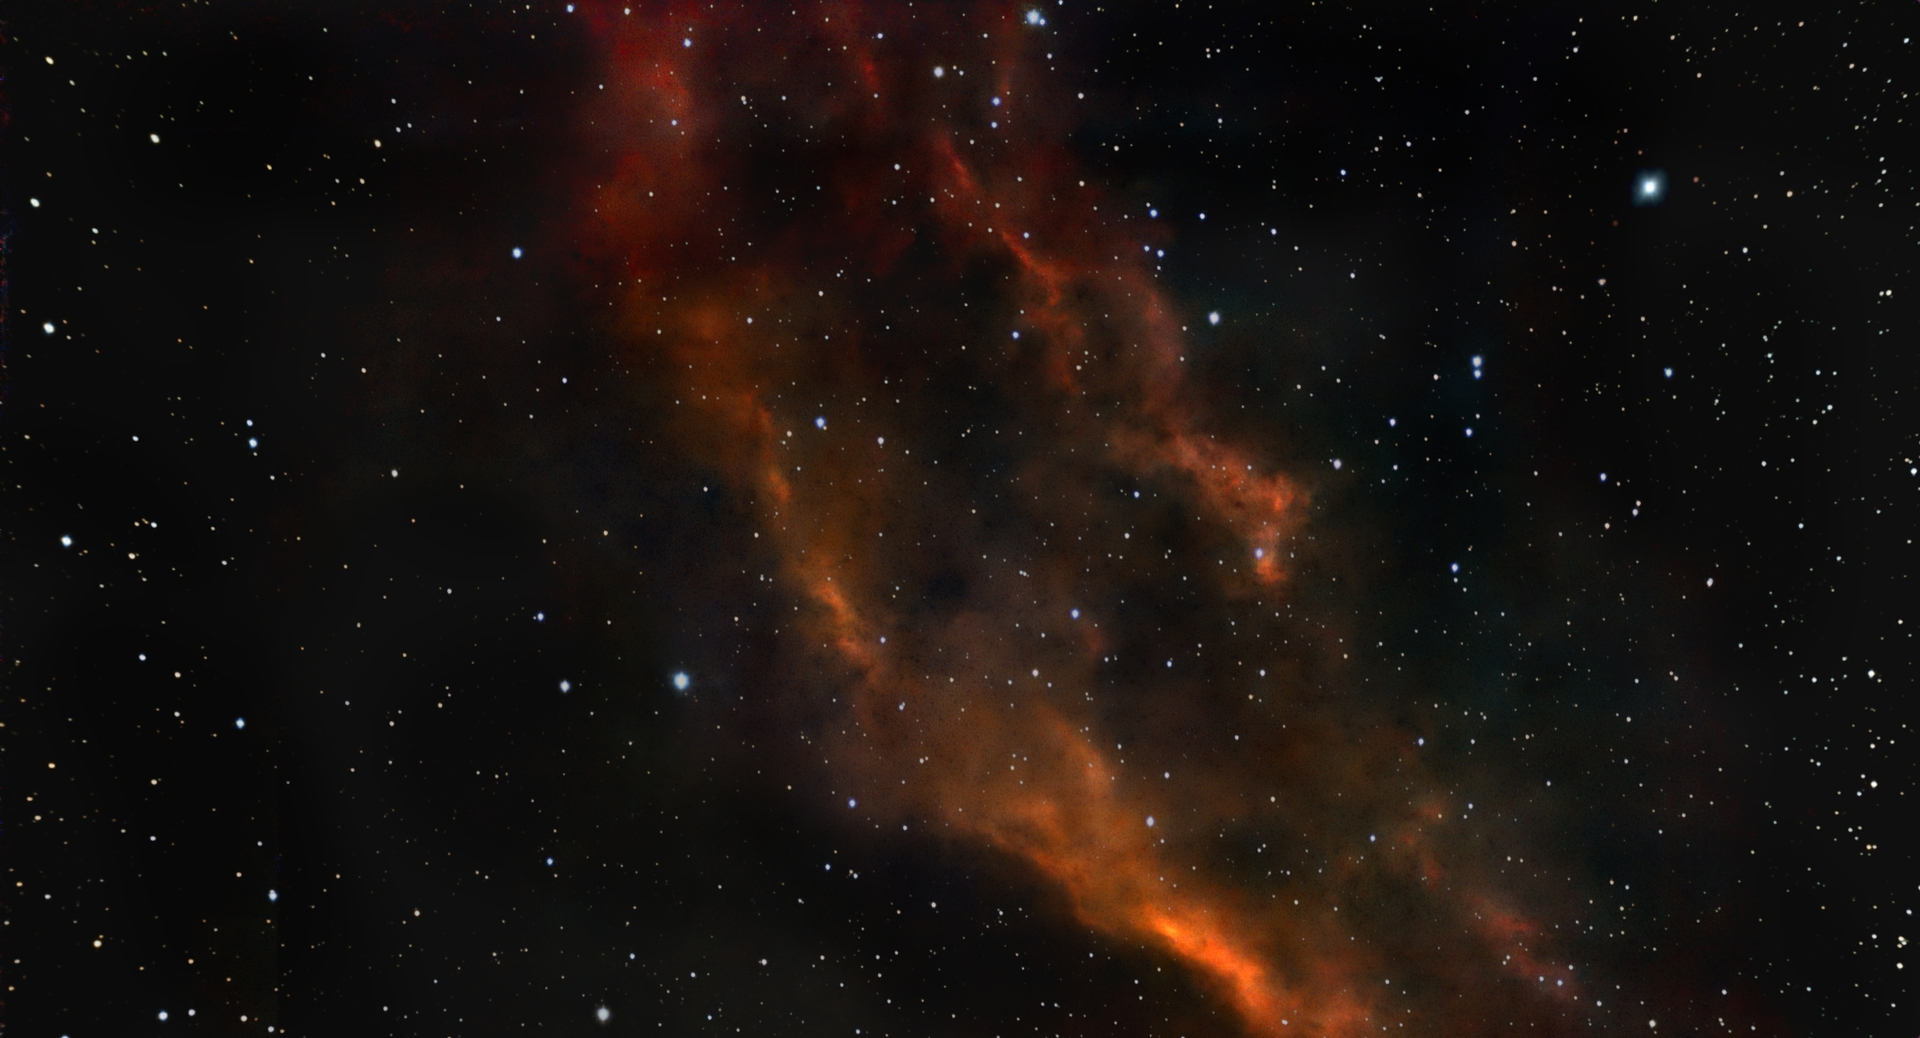
\includegraphics[width=\textwidth]{/home/lcv/Dropbox/AstroPhotography/Imaging/Original/California_Nebula.jpg}
{\footnotesize\color{white}
The Andromeda Galaxy is a barred spiral galaxy and is the nearest major galaxy to the Milky Way. It was originally named the Andromeda Nebula and is cataloged as Messier 31, M31, and NGC 224. Andromeda has a D25 isophotal diameter of about 46.56 kiloparsecs (152,000 light-years)[8] and is approximately 765 kpc (2.5 million light-years) from Earth. The galaxy's name stems from the area of Earth's sky in which it appears, the constellation of Andromeda, which itself is named after the princess who was the wife of Perseus in Greek mythology. \myhttp{Wikipedia}{https://en.wikipedia.org/wiki/Andromeda_Galaxy}
}
\section{Eagle Nebula}
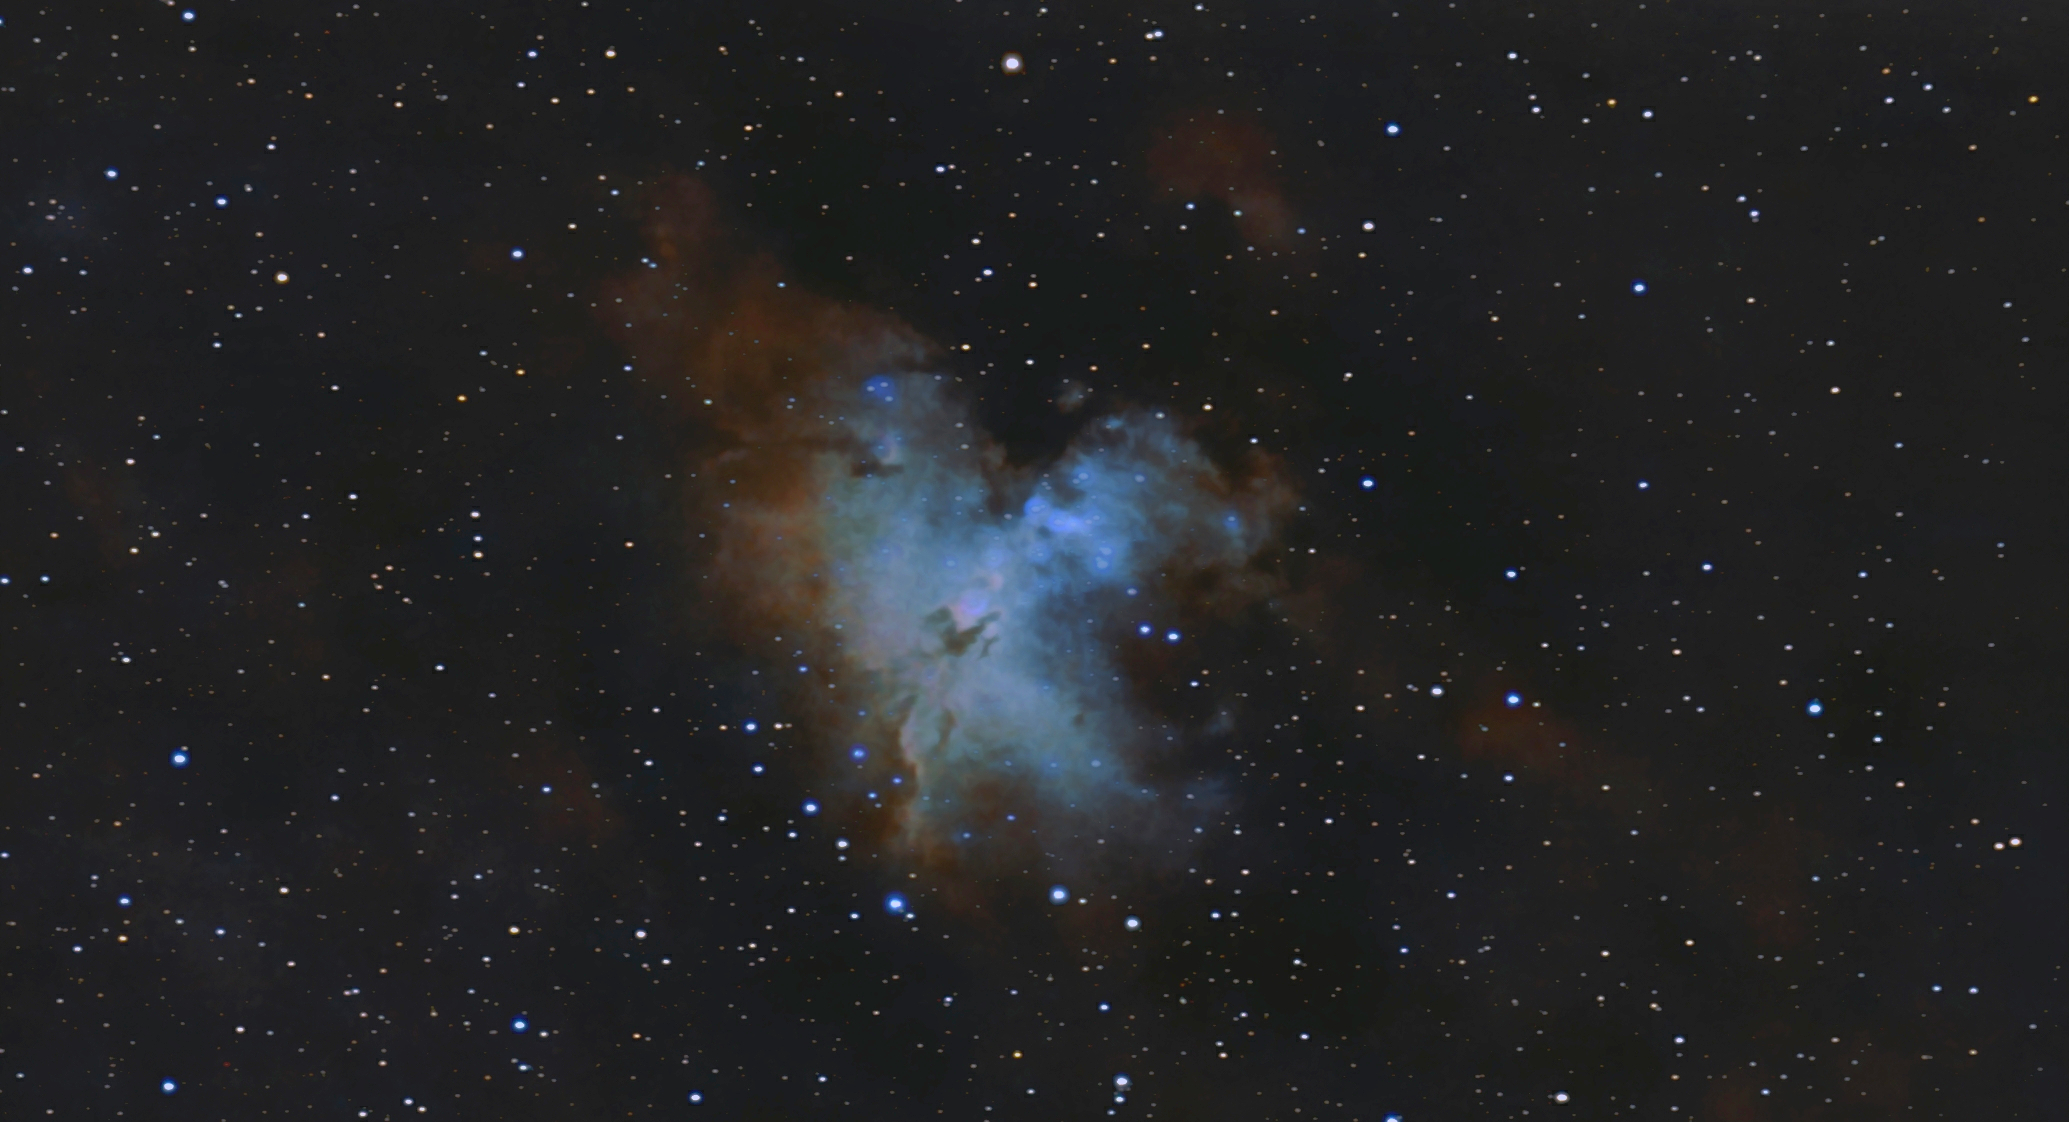
\includegraphics[width=\textwidth]{/home/lcv/Dropbox/AstroPhotography/Imaging/Original/Eagle_Nebula.jpg}
{\footnotesize\color{white}

}
\section{Eastern Veil Nebula}
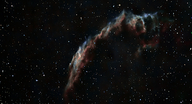
\includegraphics[width=\textwidth]{/home/lcv/Dropbox/AstroPhotography/Imaging/Original/Eastern_Veil_Nebula.jpg}
{\footnotesize\color{white}

}
\section{Fireworks Galaxy}
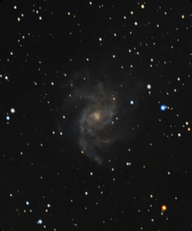
\includegraphics[width=\textwidth]{/home/lcv/Dropbox/AstroPhotography/Imaging/Original/Fireworks_Galaxy.jpg}
{\footnotesize\color{white}

}
\section{Ghost Of Cassiopeia}
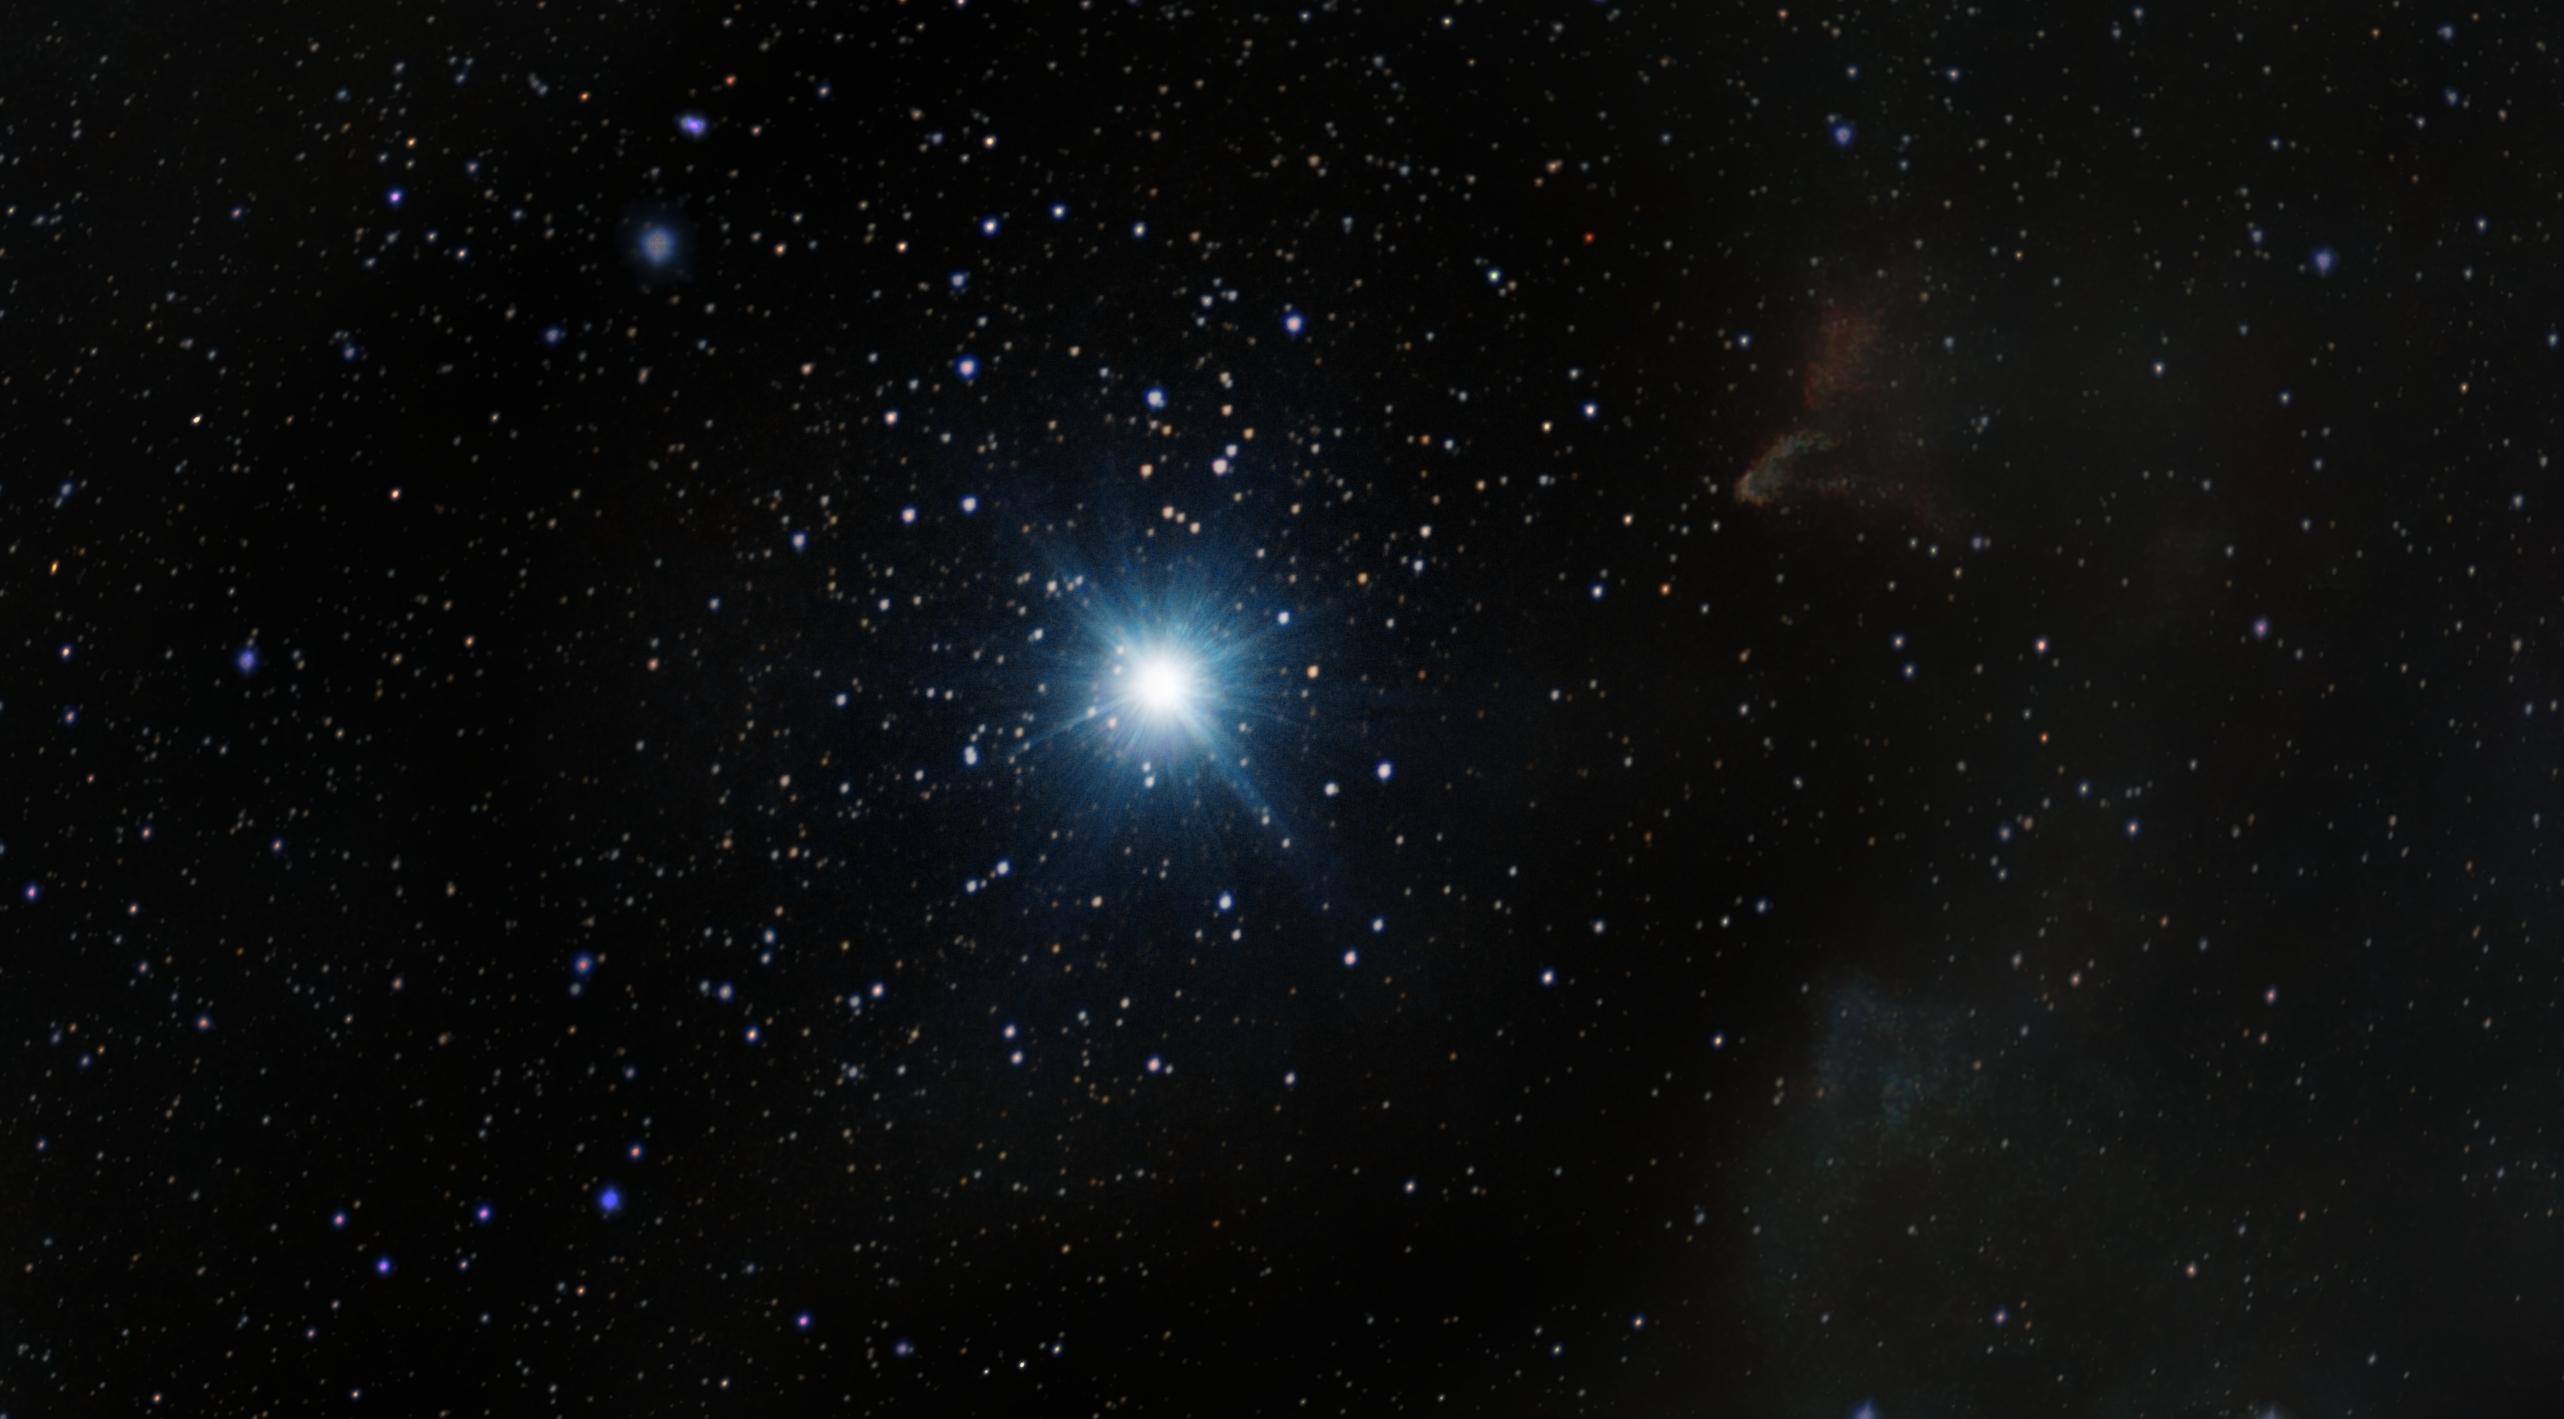
\includegraphics[width=\textwidth]{/home/lcv/Dropbox/AstroPhotography/Imaging/Original/Ghost_Of_Cassiopeia.jpg}
{\footnotesize\color{white}

}

